\documentclass[9pt, compress, blue]{beamer}
\mode<presentation>
\usetheme{Warsaw}
%\usetheme{Hannover}
%\usecolortheme{lily}
\useoutertheme[subsection=false]{smoothbars}
%\useinnertheme{rectangles}
%\hypersetup{pdfpagemode=FullScreen} % makes your presentation go automatically to full screen
\setbeamertemplate{footline}[text line]{} % makes the footer EMPTY

%\usetheme{Hannover}
%\usetheme{default}
\definecolor{links}{HTML}{2A1B81}
\hypersetup{colorlinks,linkcolor=,urlcolor=links}
\usepackage{listings}
\usepackage{wrapfig}
\usepackage{mdwlist}
\usepackage{subfigure}
\usepackage[normalem]{ulem}

\newcommand{\deriv}[2]{\frac{\partial {#1}}{\partial {#2}}}
\newcommand{\xx}{{\bf x}}
\newcommand{\dx}{\delta \xx}

\usepackage{tikz}
\tikzstyle{node}=[draw, circle,bottom color=black!25, top color = gray!25, minimum size=20pt,inner sep=0pt]
\tikzstyle{job}=[draw, circle, bottom color=red!25, top color = orange!25, minimum size=20pt,inner sep=0pt]
\tikzstyle{edge} = [draw,thick,-]
\tikzstyle{weight} = [font=\small]

\begin{document}

%=======================================================================
\begin{frame}{APE - Array Primitives}

\textbf{Desire:} 1000 line C programs are challenging to optimize. \\
Our problems are well structured and can be expressed more concisely 
This can facilitate otherwise infeasible optimization
\vspace{10pt}

\textbf{Goal:} Find a small set of operations that describe our problems well.
\vspace{10pt}

\textbf{Our Solution:} Array Primitives 
\vspace{10pt}

\textbf{Reasoning:} They form a particularly nice interface between
programmer and hardware. 
\begin{itemize}
\item Hails from a familiar and well used syntax (MatLab)
\item Well tuned software packages exist on a variety of architectures \\
(i.e. BLAS/LAPACK implemented for both CPUs and GPUs) 
\item Relatively predictable operation costs (memory and time) \\
As a result optimization is easy
\item Forms a connection to Linear Algebra
\item Lots of work already done by the Theano project
\end{itemize}

\end{frame}
%=======================================================================
\begin{frame}[fragile]{APE - Current Proect} 
Can a computer schedule HPC code?
\begin{lstlisting}
>>> x = T.matrix('x')
>>> y = x*x
>>> z = y.sum()
\end{lstlisting}
Computation Graph
\begin{figure}
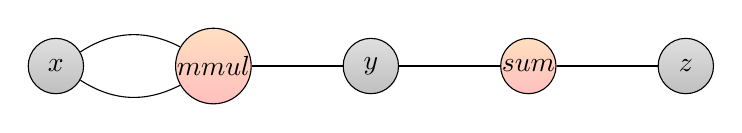
\begin{tikzpicture}[scale=2, auto,swap]
    \foreach \pos/\name in {
                            {(0, 0)/x},
                            {(2,0)/y}, 
                            {(4,0)/z}}
        \node[node] (\name) at \pos {$\name$};

    \foreach \pos/\name in {
                            {(1,0)/mmul}, 
                            {(3,0)/sum}}
        \node[job] (\name) at \pos {$\name$};

    % Connect vertices with edges and draw weights
    \draw (x) to[bend right] (mmul);
    \draw (x) to[bend left] node[weight] {}(mmul);
    \draw (y) -- (sum);
    \draw (mmul) -- (y);
    \draw (sum) -- (z);

\end{tikzpicture}
\end{figure}
Architecture Graph
\begin{figure}
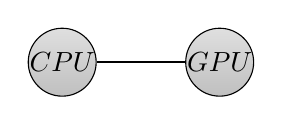
\begin{tikzpicture}[scale=2, auto,swap]
    \foreach \pos/\name in {
                            {(0,0)/CPU},
                            {(1,0)/GPU}}
        \node[node] (\name) at \pos {$\name$};

    % Connect vertices with edges and draw weights
    \foreach \source/ \dest /\weight in {CPU/GPU/1}
        \path[edge] (\source) -- node[weight] {} (\dest);

\end{tikzpicture}
\end{figure}
We have implementations for all operations on both CPU and GPU as well as
predictable runtimes. Finding optimal schedules for problems of this size is
easy. 

\end{frame}
%=======================================================================

\begin{frame}{APE -- Can we go bigger?}
\begin{figure}[ht]
\vspace{-0pt}
\centering
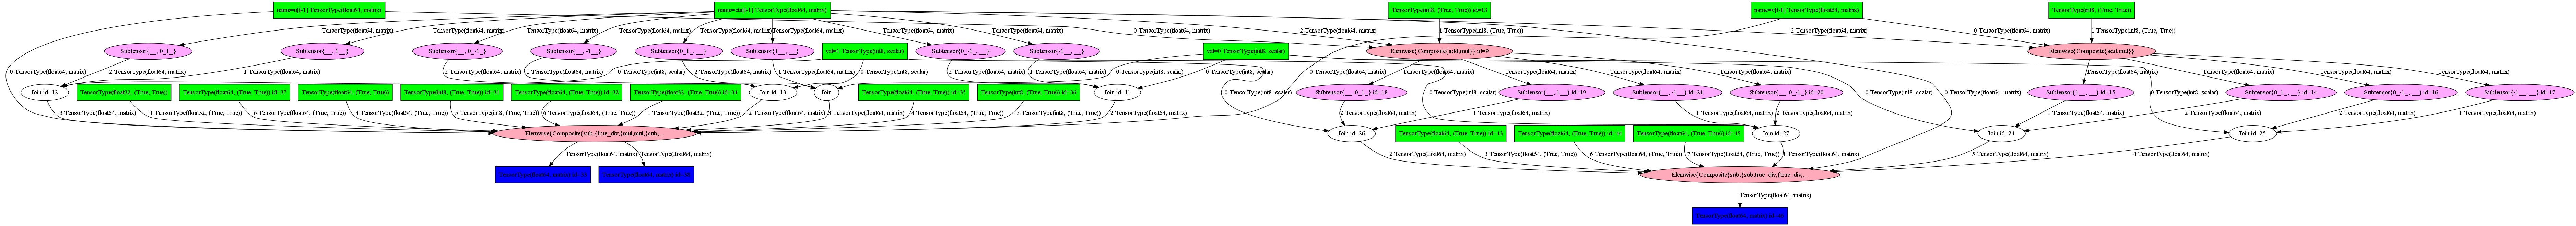
\includegraphics[width=\textwidth]{f_timeEvolutionScanOp_18}
\end{figure}
\vspace{-10pt}

\begin{columns}
\column{.4\textwidth}
Time step for the shallow water equations, solved
by a finite difference scheme on a regular grid with periodic boundary
conditions.

\column{.6\textwidth}
\begin{figure}[ht]
\vspace{-0pt}
\centering
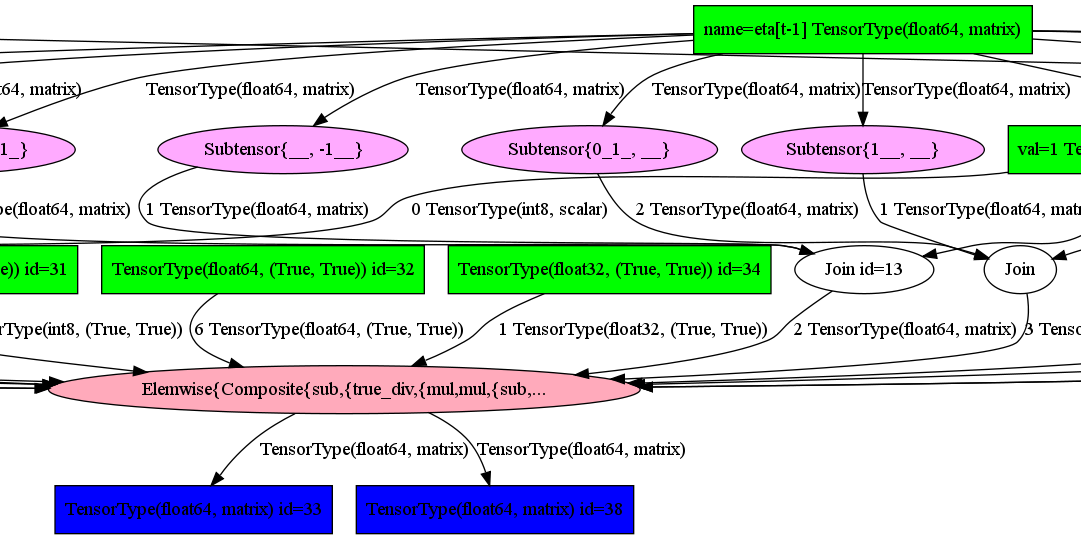
\includegraphics[width=\textwidth]{f_timeEvolutionScanOp_18_cropped}
\vspace{-0pt}
\vspace{00pt}
\end{figure}
\end{columns}

\vspace{-7pt}

\begin{columns}
\column{.6\textwidth}
Can we effectively schedule moderate sized problems?
\begin{itemize}
\item ILP scheduling is solvable at this scale\\ (slow but feasible)
\item Approximation algorithms to ILP are well studied
\item Heuristics exist in OR and embedded systems communities
\end{itemize}
\column{.4\textwidth}
\begin{figure}
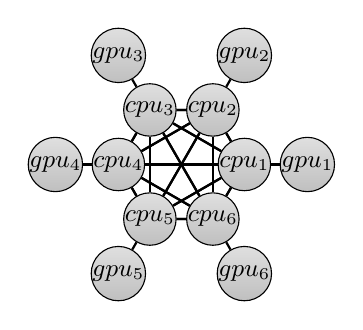
\begin{tikzpicture}[scale=.8, auto,swap]
    \tikzstyle{cpu}=[draw, circle,bottom color=black!25, top color = gray!25,
        minimum size=1pt,inner sep=0pt, font=\small]
    \tikzstyle{gpu}=[draw, circle,bottom color=black!25, top color = gray!25,
        minimum size=1pt,inner sep=0pt, font=\small]

  \foreach \name/\angle in {cpu_1/0, cpu_2/60, cpu_3/120, cpu_4/180, cpu_5/240,
                            cpu_6/300}
        \node[cpu] (\name) at (\angle:1cm) {$\name$};
  \foreach \name/\angle in {gpu_1/0, gpu_2/60, gpu_3/120, gpu_4/180, gpu_5/240,
                            gpu_6/300}
        \node[gpu] (\name) at (\angle:2cm) {$\name$};
  \foreach \a in {cpu_1, cpu_2, cpu_3, cpu_4, cpu_5, cpu_6}
      \foreach \b in {cpu_1, cpu_2, cpu_3, cpu_4, cpu_5, cpu_6}
          \path[edge] (\a) -- node[weight] {} (\b);
  \foreach \cpu/\gpu in {cpu_1/gpu_1, cpu_2/gpu_2, cpu_3/gpu_3, cpu_4/gpu_4,
                         cpu_5/gpu_5, cpu_6/gpu_6}
          \path[edge] (\cpu) -- node[weight] {} (\gpu);


\end{tikzpicture}
\end{figure}
\end{columns}
\end{frame}


%=======================================================================
\begin{frame}{APE - Future Questions}

This may be useful for moderate sized problems. Can this way of thinking be
extended to larger issues? 

\begin{itemize}
\item Can we extend this to large distributed problems/systems?
\item Can we build optimized operations for specific hardware? \\
I.e. can we build a good sparse MatVec for BlueGene
\item Can we then use these operations as primitives in another layer? 
\item What other domains use array based operations. Can we engage them?
\item At what other levels might we want to build compilers? Linear Algebra?
\item Can we build a stack of compilers \\
\textit{gcc/nvcc $\rightarrow$ APE $\rightarrow$ Linear Algebra $\rightarrow$
PDEs} \\
such that we optimize a problem of moderate complexity at each step. 
\end{itemize}
\end{frame}


\end{document}
